\documentclass[12pt]{article}
\usepackage[utf8]{inputenc}
\usepackage[T1]{fontenc}
\usepackage[norsk]{babel}
\usepackage{amsmath}
\usepackage{amsthm}
\usepackage{amsfonts}
\usepackage{amssymb}
\usepackage{enumerate}
\usepackage{physics}
\usepackage{graphicx}
\usepackage{wrapfig}
\usepackage{float}

\usepackage[top=0.4in, bottom=0.4in, left=0.4in, right=0.4in]{geometry} % Reduce margins

\begin{document}
\section{Energi i termofysikk}
\subsection{Ideell gass}
For lav-tetthets gasser gjelder
\begin{align*}
  PV = NkT = nRT
\end{align*}
\subsection{Ekvipartisjon av energi}
Gjelder for alle energiformer der formelen er en kvadratisk funksjon av koordinat-
eller hastighetskomponent. Dersom det i et system er $N$ molekyler med $f$
frihetsgrader hver, ingen ikke-kvadratiske temperaturavhengige former for energi
er den midlere (totale for store $N$) termiske energien gitt ved
\begin{align*}
  U_\text{termisk} = N f \frac{1}{2}kT
\end{align*}
Tar ikke hensyn til for eksempel hvileenergi, så tryggest å bruke for endringer
i energi med endringer i temperatur, og unngå tilfeller med faseoverganger
eller andre reaksjoner der kjemiske bindinger frigjør/krever energi.

\subsubsection{Telling av frihetsgrader}
Telling av frihetsgrader. Monoatomisk gass: Kun translasjonell bevegelse i tre
dimensjoner gir frihetsgrader, så $f = 3$. Diatomisk gass: Translasjonell
bevegelse i 3D + rotasjon om to akser (aksen gjennom lengden av molekylet
teller ikke pga. kvantemekanikk), så $f = 5$. Polyatomiske molekyler kan som
regel roteres om tre akser, som gir det siste rotasjonsbidraget. Vibrasjon
gir både kinetisk og potensiell energi bidrag, altså øker frihetsgraden med to.
Ved romtemperatur bidrar ikke vibrasjon til termisk energi, ved høyere temperaturer
kommer dette bidraget inn.

I et fast stoff kan atomer vibrere i tre ortogonale retninger, som gir 6 frihetsgrader.
Noen av disse kan "fryses ut" ved romtemperatur. Væsker er som regel mer kompliserte,
ekvipartisjonsteoremet gjelder for translasjonell bevegelse, men ikke for andre
bidrag siden de er ikke-kvadratiske.

\subsection{Varme og arbeid}
Overføringer av energi klassifiseres på to måter: \newline \noindent
\textbf{Varme}: overføring av energi fra et objekt til et annet på grunn av innbyrdes forskjell i temperatur. Ledning (molekylær
kontakt), konveksjon (bevegelse av områder av gass/væske) og elektromagnetisk stråling.\newline \noindent
\textbf{Arbeid} er enhver annen overføring av energi inn eller ut av et system.
\newline \noindent
Endringen i energi for et system er summen av varme og arbeid (termodynamikkens første lov)
\begin{align*}
  \Delta{U} = Q + W
\end{align*}
\subsection{Kompresjonsarbeid}
Arbeid som behøves for å redusere et volum av gass (trykk $P$) $\Delta V$ ved
\textbf{kvasistatisk} kompresjon (gassen rekker hele tiden å justere til likevekt).
\begin{align*}
  W = -P \Delta{V} \quad (\text{ved } P \neq P(V))\qquad W = - \int_{V_i}^{V_f} P(V) \dd V \quad (\text{ved } P = P(V))
\end{align*}
To idealiserte kompresjonstyper for ideell gass: \textbf{isotermal kompresjon}
(så sakte at temperatur i gassen er uendret) og \textbf{adiabatisk kompresjon}
(så kjapp at ingen varme slipper ut av systemet i prosessen). \newline \noindent
\textbf{Isotermal kompresjon}: Kvasistatisk, så
\begin{align*}
  W = -\int_{V_i}^{V_f} P \dd V = -NkT \int_{V_i}^{V_f} \frac{1}{V} \dd V = NkT \ln{\frac{V_i}{V_f}}
\end{align*}
Samme energi slipper ut ved varme (vises med første lov).\newline \noindent
\textbf{Adiabatisk kompresjon}: Ingen varme unnslipper, $\Delta U = Q + W = W$.
Bruk ekvipartisjon $\dd U = \frac{f}{2} N k \dd T$ og kvasistatisk kompresjon,
bruk ideell gass lov for trykket og løs separabel difflign. Får (med $\gamma = f(f+2)$)
\begin{align*}
  V T^{f/2} = \text{constant} \overset{\text{Ideell gass lov}}{\implies} V^\gamma P = \text{constant}
\end{align*}
\subsection{Varmekapasiteter}
Varmekapasitet defineres som $C = Q/\Delta{T}$ (varme per grad temperaturøkning). Tvetydig,
avhenger av omstendigheter (mengde stoff/gass, arbeid osv.). Derfor har man
varmekapasitet med $W = 0$ (som regel er $V$ da konstant, ingen kompressjon):
\begin{align*}
  C_V = \left( \frac{\Delta U}{\Delta T} \right)_V = \left( \pdv{U}{T}\right)_V
\end{align*}
Ofte ekspanderer gasser når de varmes opp, da tapes energi ved arbeid på omgivelsene.
Dersom det er konstant trykk i omgivelsene er
\begin{align*}
  C_P = \left( \frac{\Delta U - (-P\Delta V)}{\Delta T} \right)_P =  \left( \pdv{U}{T}\right)_P + P\left( \pdv{V}{T}\right)_P
\end{align*} \newline \noindent
\textbf{Latent varme:} Ved faseoverganger øker ikke temperaturen ved tilførsel av energi. Da
er varmekapasiteten per def uendelig: $C = Q/\Delta{T} = Q/0 = \infty$. Energien som kreves
for å fullføre faseoverangen kalles den latente varmen $L = Q/m$, og er varmen per
masse som kreves.\newline \noindent
\textbf{Entalpi:} Entalpi er energien til et system + ekspansjonsarbeidet som
krevdes for å putte det i det systemet det er i: $H = U + PV$. Observer at
$C_P = \left( \pdv{H}{T} \right)_P$.
\subsection{Prosesshastigheter (rates of processes)}
Orker ikke dette nå.
\section{Termodynamikkens andre lov}
\subsection{To tilstands systemer - paramagnetisme}
\textbf{Mikrotilstand} er alle partiklenes tilstander, \textbf{makrotilstand} sier
noe mer generelt om systemet. Multiplisiteten $\Omega(s)$ til en makrotilstand $s$ er antallet mikrotilstander
tilhørende makrotilstanden. Sannsynligheten for en makrotilstand er $\Omega(s)/\Omega(\text{alle})$. I en
to-tilstands paramagnet kan spinnene peke opp eller ned, $N = N_\uparrow + N_\downarrow$ er det totale antallet
spinn.
\begin{align*}
  \Omega(N_\uparrow) = \binom{N}{N_\uparrow} = \frac{N!}{N_\uparrow! (N - N_\uparrow)!} = \frac{N!}{N_\uparrow N_\downarrow}
\end{align*}
\subsection{Einsteinmodellen for faste stoffer}
System med et vilkårlig antall energi "enheter", alle med samme størrelse. Dette
er tilfellet for harmonisk oscillator, med steg $hf$ (Referansenivå settes til 0).
Disse oscillatorene gjelder for atomene i faste stoffer, 3 oscillatorer per atom
pga frihetsgrader. Multiplisiteten til Einstein solid med $N$ oscillatorer og
$q$ energi enheter er
\begin{align*}
  \Omega(N,q) = \binom{q + N - 1}{q} = \frac{(q + N - 1)!}{q!(N-1)!}
\end{align*}
\subsection{Interagerende systemer}
Har nå to Einstein solids, $A$ og $B$, som kan dele energi. Systemene uavhengige
av hverandre, så for en gitt energifordeling er multiplisiteten $\Omega_\text{tot} = \Omega_A \Omega_B$.\newline \noindent
\textbf{Fundamental antagelse i statistisk mekanikk:} I et isolert system i termisk
likevekt er enhver tilgjengelig mikrotilstand like sannsynlig. Merk at denne antagelsen
forutsetter at tidsskalaen er mye større enn tiden energiforskyvninger skjer. \newline \noindent
Observerer at multiplisiteten er langt høyere for de jevnere fordelingene av energi,
så med antagelsen over må en måling av jevn fordeling være overveldende sannsynlig.
\textbf{Termodynamikkens andre lov}(versjon 1): Multiplisiteten øker når et system
er for seg selv, fordi det er overveldende sannsynlig.
\subsection{Store systemer}
\subsubsection{Veldig store tall}
\textbf{Små tall:} 2,6,98. \textbf{Store tall:} Eksponentiering av små tall, f.eks
Avogadros tall $\sim 10^{23}$. Regneregel: $10^{23} + 23 = 10^{23}$.
\textbf{Veldig store tall:} Eksponentiering av store tall, f.eks $10^{10^{23}}$.
Regneregel: $10^{10^{23}} \times 10^{23} = 10^{(10^{23} + 23)} = 10^{10^{23}}$.
Logartime gjør et veldig stort tall til et stort tall osv, dette brukes mye.
\subsubsection{Stirlings Approksimasjon}
\begin{align*}
  N! \approx N^N e^{-N}\sqrt{2\pi N}
\end{align*}
Korrekt i grensen $N \gg 1$. God approksimasjon for logaritmen er gitt som $\ln{N!} \approx N \ln N - N$.
\subsubsection{Multiplisiteten til et stort Einstein solid}
Bruk Stirling på multiplisiteten til Einstein solid, med en rekkeutvikling av en
logaritme underveis. I grensen $q \gg N$ fåes
$\Omega(N,q) \approx \left(\frac{eq}{N}\right)^N$
\subsubsection{Skarpheten til multiplisitetsfunksjonen}
For to interagerende Einstein solids med $q \gg N$ er $\Omega = \left(\frac{e}{N}\right)^{2N} (q_A q_B)^{2N}.$
Har en skarp topp ved $\Omega = (e/N)^{2N} (q/2)^{2N}$, altså $q_A = q_B = q/2$,
en lik fordeling av energi. Fordelingen er Gaussisk og bredden er gitt ved $q/\sqrt{N}$.
For store $N$ vil fluktuasjoner være umulige å måle, denne grensen kalles den \textbf{termodynamiske grensen}.
\subsection{Ideell gass}
Utledning viser at $\Omega(U,V,N) \approx f(N) V^N U^{3N/2}$, der $f(N) = \frac{1}{N!} \frac{1}{h^{3N}} \frac{\pi^{3N/2}}{(3N/2)!} (2m)^{3N/2}$.
Kombineres to av disse (kun energiutveksling) fåes $\Omega_\text{total} = [f(N)]^2 (V_A V_B)^2 (U_A U_B)^{3N/2}$,
samme type uttrykk som for Einstein solid. Smal peak med høye multiplisiteter.
\subsection{Entropi}
Definerer entropi som (fordi multiplisitet er et veldig stort tall, og store tall er enklere å jobbe med)
\begin{align*}
  S = k \ln{\Omega}
\end{align*}
Dimensjon energi per temperatur, enhet $J/K$. En nyttig egenskap: $S_\text{tot} = k \ln{\Omega_\text{tot}} = k \ln{(\Omega_A \Omega_B)} = S_A + S_B$. \newline \noindent
\textbf{Termodynamikkens andre lov:} Ethvert stort system i likevekt vil være i
makrotilstanden med størst entropi (utenom fluktuasjoner som vanligvis er for små
til å måle). Altså: Entropi har en tensens til å øke.
\\ \\
Entropi kan ikke reduseres, enhver reduksjon i entropi i et system har skapt
mer entropi utenfor systemet.
\subsubsection{Entropi for en ideell gass}
\subsubsection{Blandingsentropi}
\section{Interaksjoner og implikasjoner}
\subsection{Temperature}
Se på system med to Einstein solids med noen hundre oscillatorer hver som deler
100 enheter energi. Plott entropi (individuelle og total) mot energi. Observer at
ved likevekt er $\pdv{S_A}{U_A} + \pdv{S_B}{U_A} = 0 \implies \pdv{S_A}{U_A} = \pdv{S_B}{U_B}$.
Dvs. det som er likt for begge systemer når de er i likevekt er stigningstallet til
entropi mot energigrafene, som da må ha noe med temperatur å gjøre (siden det er slik
temperatur er definert). Observer videre at det systemet med lav energi (da har det andre høy energi)
har en brattere $S$ mot $U$ graf, så en økning i energi skaper mer entropi enn det
høy energi systemet mister, så denne prosessen skjer av seg selv ifølge den andre loven.
Høyt stigningstall korresponderer med lav temperatur, og lavt med høy temperatur. Dette gir:
\begin{align*}
  \frac{1}{T} = \left(\pdv{S}{U} \right)_{N,V}
\end{align*}
\subsection{Entropi og varme}
\subsubsection{Finne termodynamiske størrelser for et system}
\begin{enumerate}
  \itemsep0em
  \item Bruk kvantemekanikk og/eller kombinatorikk til å finne et uttrykk for
  multiplisiteten som funksjon av $U,V,N$ og/eller andre variable. Må ofte bruke
  Stirlings approksimasjon og se på grenser.
  \item Ta logaritmen for å finne entropien.
  \item Deriver entropi mhp. energi for å finne temperatur som funksjon av $U$
  og evt. andre variable.
  \item Deriver $U(T)$ med hensyn på $T$ for å finne varmekapasiteten (med andre
  variable holdt konstant). Gjør andre operasjoner for å finne andre variable.
\end{enumerate}
\subsubsection{Måle entropier}
\subsubsection{Makroskopisk syn på entropi}
\subsection{Paramagnetisme}
$N$ spin 1/2 dipoler. $N_\uparrow: q = -\mu B$ og $N_\downarrow: q = \mu B$.
Total energi $U = N_\uparrow(-\mu B) + N_\downarrow \mu B = \mu B(N_\downarrow - N_\uparrow) = \mu B(N - 2N_\uparrow)$.
Magnetisering $M = \mu(N_\uparrow - N_\downarrow) = \frac{-U}{B}$. Brukes Stirling
på multiplisitetsfunksjonen og stegene over fåes $U = -N\mu B\tanh{\left(\frac{\mu B}{kT} \right)}$.
\subsection{Mekanisk likevekt og trykk}
Hva med når systemer $A$ og $B$ kan utveksle både energi og volum? Utveksling av
energi skjer på grunn av temperaturer, utveksling av volum styres av trykk.
Ved likevekt er $\pdv{S}{V_A} = 0$ (også ingen endring med hensyn på energi). Trykket
må være likt i begge sider ved likevekt, og ved stor endring i entropi per endring i
volum vil trykket være stort, gassen ønsker å ekspandere. Relasjonen blir
\begin{align*}
  P = T \left( \pdv{S}{V} \right)_{U,N}
\end{align*}
\subsubsection{Den termodynamiske identiteten}
Anta det skjer en prosess på et system der energien og volumet endres med $\Delta U$
og $\Delta V$ (volum konstant under energiendring, energi konstant under volumendring).
Prosessen kan deles opp i to steg, og endringen i entropi er gitt ved summen av
endringene fra de to prosessene. Så ved identitetene over er
\begin{align*}
  \dd S = \left( \pdv{S}{U} \right)_{V} \dd U + \left( \pdv{S}{V} \right)_{U}\dd V
\end{align*}
Dette kalles \textbf{den termodynamiske identiteten}, og skrives ofte om til (merk
at disse ligningene forutsetter at andre variable, som $N$, holdes konstant)
\begin{align*}
  \dd U = T \dd S - P \dd V
\end{align*}
\subsubsection{Entropi og varme igjen}
Uttrykket over ligner veldig på $\dd U = Q + W$ (termodynamikkens første lov).
Sammenligningen gjelder så lenge volumendringer skjer kvasistatisk og andre
størrelser er konstante (f.eks $N$). Da er $W = -P \dd V$, så $Q = T \dd S$,
selv om det gjøres arbeid på systemet. I tilfellet der endringen er adiabatisk $Q = 0$
og kvasistatisk er entropien uendret. Dette kalles en \textbf{isentropisk} prosess.
\subsection{Diffusiv likevekt og kjemisk potensial}
To systemer i termisk likevekt har like temperaturer. Mekanisk likevekt tilsvarer
like trykk. Hva med diffusiv likevekt? Betrakt to systemer som kan utveksle
partikler og energi, men er under konstant volum. Antar samme "art", f.eks $\text{H}_2\text{O}$,
men tilstandsformer er vilkålig. Antar total energi og antall partikler er konstant,
så ved likevekt er $\left( \pdv{S}{U_A} \right)_{N_A, V_A} = 0$ og $\left( \pdv{S}{N_A} \right)_{U_A, V_A} = 0$.
Ved likevekt er $\pdv{S}{N_A} = \pdv{S}{N_B}$ ved konstant energi og volum. Ganger opp
med temperatur og definerer det kjemiske potensialet
\begin{align*}
  \mu \equiv - T \left(\pdv{S}{N} \right)_{U,V}
\end{align*}
Systemer overlatt til seg selv vil dermed gå mot lavere kjemiske potensial, siden
dette gir høyere entropi. Altså strømmer partikler fra systemer med høyere $\mu$
til lavere.

Vi kan nå utvide den termodynamiske identiteten ytterligere. Total endring i entropi
ved å endre $U$ med $\dd U$, $P$ med $\dd P$ og $N$ med $\dd N$ er
\begin{align*}
  \dd S &= \left( \pdv{S}{U} \right)_{N, V} \dd U + \left( \pdv{S}{V} \right)_{N, U} \dd V + \left( \pdv{S}{N} \right)_{U, V} \dd N\\
        &= \frac{1}{T} \dd U + \frac{P}{T} \dd V + \mu \dd N
\end{align*}
Eller, løst for $\dd U$ fåes
\begin{align*}
  \dd U = T \dd S - P \dd V + \mu \dd N
\end{align*}
De to siste leddene kalles vanligvis henholdsvis mekanisk og kjemisk arbeid, det
første leddet er som tidligere varme. Dersom det er flere typer partikler/atomer
har de hvert sitt kjemiske potensial, da erstattes det siste leddet av en sum
av $\mu_i \dd N_i$ ledd.
\section{Motorer og kjølemaskiner}
\subsection{Varmekraftmaskiner}
En \textbf{varmekraftmaskin} er et apparat som absorberer varme og omdanner
deler av energien til arbeid. Et eksempel er dampturbinen. Grunnen til at kun
deler av energien kan omdannes er at når varme strømmer inn kommer det også
entropi, og denne må en kvitte seg med før prosessen kan starte om.
\begin{wrapfigure}{R}{0.4\textwidth}
  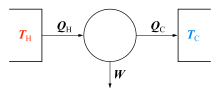
\includegraphics[width=0.3\textwidth]{figures/carnot.png}
\end{wrapfigure}
Varme kommer fra det \textbf{varme reservoiret} $T_H$ og varmen som dumpes dumpes til
det \textbf{kalde reservoiret} $T_C$. Arbeidet motoren gjør er $W$. Alle størrelsene er positive.
Effektivitet defineres som arbeid ut per varme inn
\begin{align*}
  e \equiv \frac{W}{Q_h}
\end{align*}
Hvordan maksimere effektiviteten? Energibevaring gir $Q_h = Q_c + W$, som gir
effektiviteten $e = \frac{Q_h - Q_c}{Q_h} = 1 - Q_c/Q_h$.

Videre, entropien i systemet kan ikke bli mindre, så $Q_c / T_c \geq Q_h / T_h$.
Settes dette inn i effektivitetsuttrykket over får man $e \leq 1 - T_c / T_h$.
Velg $T_c$ og $T_h$ slik at forholdet blir så lite som mulig. Den første loven
sier 'du kan ikke vinne', og den andre loven sier at 'du går uansett i underskudd'.
\subsubsection{Carnotsyklusen}

\subsection{Kjølemaskiner}
Kjølemaskiner er varmekraftmaskiner kjørt baklengs. Varme går fra det kalde
reservoiret til det varme ved tilførsel av arbeid som elektrisk energi. Kjøleskapet
er det kalde reservoiret og systemet utenfor det varme. 'Søppelvarme' dumpes ut
i kjøkkenet. COP (coefficient of performance) defineres som
\begin{align*}
  \text{COP} = \frac{\text{benefit}}{\text{cost}} = \frac{Q_c}{W}
\end{align*}
Kan som over bruke første og andre lov til å vise begrensninger for COP.
\section{Fri energi og kjemisk termodynamikk}
\subsection{Fri energi som tilgjengelig arbeid}
\textbf{Entalpi} er energien til et system pluss arbeided som behøves for å lage plass ved å dytte
atomosfære/annet med trykk $P$ vekk. Altså energi som trengs hvis systemet
skal dannes ut av intet og plasseres i et annet system:
\begin{align*}
  H \equiv U + PV
\end{align*}
\textbf{Helmoholtz fri energi} er energien som trengs for å lage et system, minus
varmen man får 'gratis' fra omliggende atmosfære med temperatur $T$. Ekvivalent er
dette energien som kan hentes ut dersom systemet annihileres, entropi kan ikke minke
så entropi må dumpes ut som varme. $F$ er da energien man får ut som arbeid:
\begin{align*}
  F \equiv U - TS
\end{align*}
\textbf{Gibbs fri energi} er en kobinasjon av de over.
\begin{align*}
  G \equiv U - TS + PV
\end{align*}
Som regel betraktes ikke situasjoner der hele systemet annihileres, så det er
bedre å se på endringer i størrelsene over. Da er $\Delta F = \Delta U - T \Delta S = Q + W - T \Delta S$.
Dersom ingen entropi dannes er $Q = T\Delta S$, og $\Delta F = W$. Dersom entropi
dannes er $T\Delta S > Q$, og $\Delta F < W$, så ved konstant temperatur er
\begin{align*}
  \Delta F \leq W
\end{align*}
Samme argumentasjon for konstant trykk og temperatur og at $W = -P\Delta V + W_\text{annet}$
gir
\begin{align*}
  \Delta G \leq W_\text{annet}
\end{align*}
\subsubsection{Elektrolyse, brenselceller og batterier}
Et eksempel på bruk av $\Delta G$, betrakt reaksjonen $\text{H}_2 \text{O} \rightarrow \text{H}_2 + \frac{1}{2}\text{O}_2$,
elektrolyse av vann til hydrogen og oksygengass. Fra tabell er $\Delta H = 286$ kJ (energien man ville fått dersom man brant et mol hydrogen).
I denne reaksjonen må denne energien altså tilføres, $P\Delta V = 4$ kJ av energien går til å dytte atmosfære vekk, resten blir værende i systemet.
Hvor mye må tilføres ved arbeid og hvor mye ved varme? Fra tabeller er $S_{\text{H}_2 \text{O}} = 70 \text{ J/K}$, $S_{\text{H}_2} = 131 \text{ J/K}$
og $S_{\text{O}_2} = 205 \text{ J/K}$. Endring i entropi er $\Delta S = S_1 - S_0 = (131 + 0.5 \cdot 205) - 70 = 163$ J/K, entropien øker. Maksimal
energiendring ved varme er da $T\Delta S = 49$ kJ. Energien som behøves via elektrisk arbeid
er forskjellen $286 - 49 = 237$ kJ. Dette er endringen i Gibbs fri energi, det minste arbeidet som behøves for
å få reaksjonen til å gå: $\Delta G = 237 \text{ kJ} = \Delta H - T \Delta S = 286 \text{ kJ} - (298 \text{ K})(163 \text{ J/K})$.
\subsubsection{Termodynamiske identiteter}
Kan lage identiteter for de overnevnte energiene, betrakt små endringer i $H, U, P$ og $V$
og bruk den termodynamiske identiteten til å eliminere $\dd U$. Gir
\begin{align*}
  \dd H &= T \dd S + V \dd P + \mu \dd N \\
  \dd F &= -S \dd T - P \dd V + \mu \dd N \\
  \dd G &= -S \dd T + V \dd P + \mu \dd N
\end{align*}
Fra disse kan en rekke partiellderiverte relasjoner finnes. For eksempel
\begin{align*}
  S = -\left( \pdv{G}{T} \right)_{P,N}
\end{align*}
kan lages ved å bruke den siste og holde $P$ og $N$ konstant, dvs $\dd P = \dd N = 0$.
\subsection{Fri energi som kraft mot likevekt}
\textbf{Reservoir} av energi: System stort nok til at det kan utveksle uendelig
energi uten å endre sin temperatur. \newline \noindent
Betrakt et system med
\subsection{Faseoverganger}
En \textbf{faseovergang} er en diskontinuerlig endring i egenskapene til et stoff
når noe rundt bare endres infinitesimalt. Et \textbf{fasediagram} viser likevektsfaser
kom funksjon av trykk og temperatur. Trykket der en gass kan sameksistere med flytende
fase kalles \textbf{damptrykket}. Punktet (kombinasjonen av $P$ og $T$) der
alle tre faser sameksisterer kalles \textbf{trippelpunktet}. Ved lavere temperaturer
kan ikke væskeformen eksistere, fast stoff sublimerer til gass.
\section{Boltzmann statistikk}

\section{Kvantestatistikk}

\section{Konstanter og annet nyttig}
\subsection{Fysiske konstanter}
\begin{align*}
  k   &= 1.381 \times 10^{-23} \text{ J/K} = 6.617 \times 10^{-5} \text{ eV/K} \\
  N_A &= 6.022 \times 10^{23}        \\
  R   &= 8.315 \text{ J/mol$\cdot$K} \\
  h   &= 6.626 \times 10^{-34} \text{ J}\cdot\text{s} = 4.136 \times 10^{-15} \text{ eV}\cdot\text{s}\\
\end{align*}
\subsection{Konvertering mellom enheter}
\end{document}
